\documentclass[12pt]{article}

\usepackage{sbc-template}
\usepackage{graphicx,url}
\usepackage{amsmath}
\usepackage[utf8]{inputenc}
\usepackage[T1]{fontenc}
\usepackage[brazil]{babel}

\sloppy

\title{Degradação de Eficiência Paralela por Contenção de Cache L3 e
SMT em Processadores Híbridos: Estudo Empírico no Intel i7-13620H}

\author{Rafael Coutinho Lima\inst{1}}

\address{Bacharelado em Ciência da Computação --- CESAR School\\
  Recife --- PE --- Brasil
  \email{rcl4@cesar.school}
}

\begin{document}

\maketitle

\begin{abstract}
  This paper quantitatively investigates the impact of Simultaneous
  Multithreading (SMT/HyperThreading) and L3 cache contention on parallel
  efficiency for CPU-bound workloads on the Intel Core i7-13620H (13th
  generation, hybrid Raptor Lake-H architecture). For each thread count in
  $\{1, 2, 4, 6, 8, 10, 12, 14, 16\}$, 30 measured repetitions were collected
  after 3 discarded warm-ups, across two experiments: (A) $800 \times 800$
  matrix multiplication via \texttt{multiprocessing.Pool} (weak scaling) and
  (B) the \texttt{sysbench cpu} benchmark (strong scaling). In sysbench,
  throughput grows from 1530.0 to 13866.8 events/s from 1 to 10 threads
  (90.6\% efficiency) but plateaus at 13870.0 events/s with 16 threads --- a
  difference of only 0.02\% between 10 and 16 threads ($p = 0.804$, paired
  t-test). Per-thread efficiency drops from 90.6\% (10 threads) to 56.7\%
  (16 threads), confirming that SMT adds no extra throughput for purely
  CPU-bound work; the L3 contribution is discussed as an inferred factor. All
  data and scripts are publicly available for reproduction.

  \noindent\textbf{Keywords:} SMT; parallel efficiency; cache contention;
  hybrid processors; performance benchmarking.
\end{abstract}

\begin{resumo}
  Este artigo investiga quantitativamente o impacto do Simultaneous
  Multithreading (SMT/HyperThreading) e da contenção de cache L3 na eficiência
  de paralelismo em cargas CPU-bound no processador Intel Core i7-13620H
  (13\textsuperscript{a} geração, arquitetura híbrida Raptor Lake-H). Para cada
  número de threads em $\{1, 2, 4, 6, 8, 10, 12, 14, 16\}$ foram coletadas 30
  repetições medidas, precedidas de 3 aquecimentos descartados, em dois
  experimentos: (A) multiplicação de matrizes $800 \times 800$ via
  \texttt{multiprocessing.Pool} (weak scaling) e (B) benchmark
  \texttt{sysbench cpu} (strong scaling). No sysbench, o throughput cresce de
  1530,0 para 13866,8 eventos/s ao escalar de 1 para 10 threads (eficiência
  90,6\%), mas estagna em 13870,0 eventos/s com 16 threads --- diferença de
  apenas 0,02\% entre 10 e 16 threads ($p = 0{,}804$, teste t pareado). A
  eficiência por thread cai de 90,6\% para 56,7\%, confirmando que o SMT não
  contribui com throughput adicional em cargas puramente CPU-bound; a
  contribuição do L3 é discutida como fator inferido. Todos os dados e scripts
  estão publicamente disponíveis para reprodução.

  \noindent\textbf{Palavras-chave:} SMT; eficiência paralela; contenção de
  cache; processadores híbridos; avaliação de desempenho.
\end{resumo}

\section{Introdução}

A adoção crescente de processadores híbridos --- que combinam núcleos de alta
performance (P-cores) e núcleos de eficiência energética (E-cores) --- introduz
desafios novos na avaliação de desempenho paralelo. O Intel Core i7-13620H
(Raptor Lake-H, 13\textsuperscript{a} geração) possui 6 P-cores com SMT (12
threads lógicas) e 4 E-cores sem SMT (4 threads), totalizando 16 threads
lógicas sobre 10 núcleos físicos.

O Simultaneous Multithreading (SMT), comercialmente denominado HyperThreading
pela Intel, permite que dois threads lógicos compartilhem os recursos de
execução de um único núcleo físico. Em cargas mistas (CPU + E/S), o SMT pode
aumentar a utilização do pipeline ocultando latências de memória. Porém, em
cargas estritamente CPU-bound, dois threads lógicos competem pelos mesmos
recursos de execução, cache L1/L2 privado e entradas do TLB --- sem ganho de
throughput proporcional. Além disso, ao escalar além dos P-cores físicos, os
threads passam a compartilhar mais intensamente o cache L3 (24 MB
compartilhado), podendo causar contenção e evicções frequentes.

Este trabalho responde à seguinte pergunta de pesquisa: qual é o impacto
quantitativo do SMT e da contenção de cache L3 na eficiência de paralelismo em
cargas CPU-bound em processadores híbridos Intel de 13\textsuperscript{a}
geração? As hipóteses formais são:

\begin{itemize}
  \item \textbf{H0:} o uso de threads lógicas além dos núcleos físicos não
  degrada significativamente a eficiência paralela nem o throughput
  ($p \geq 0{,}05$).
  \item \textbf{H1:} o uso de SMT causa degradação estatisticamente
  significativa de eficiência, especialmente acima de 10 threads --- limite dos
  P-cores físicos ($p < 0{,}05$).
\end{itemize}

As contribuições deste trabalho são: (i) a quantificação empírica do plateau de
throughput causado pelo SMT em uma carga CPU-bound; (ii) a medição da
degradação de eficiência por thread acima do limite físico de P-cores; e (iii)
um conjunto de dados e scripts públicos para reprodução. O restante do artigo
está organizado em trabalhos relacionados (Seção~\ref{sec:related}), metodologia
(Seção~\ref{sec:metodo}), resultados (Seção~\ref{sec:result}), discussão
(Seção~\ref{sec:discussao}) e conclusão (Seção~\ref{sec:conclusao}).

\section{Trabalhos Relacionados}
\label{sec:related}

O conceito de multithreading simultâneo foi introduzido por \cite{tullsen1995}
no ISCA 1995, demonstrando ganhos em workloads com alta latência de memória,
mas limitações em cargas compute-bound. \cite{eyerman2009} propuseram uma
arquitetura de contabilização de ciclos por thread (\emph{per-thread cycle
accounting}) em processadores SMT, quantificando como cada thread é penalizada
ao compartilhar recursos de execução --- base para entender por que a
competição por unidades funcionais reduz os ganhos do SMT em cargas intensivas
de CPU.

A contenção por recursos compartilhados em sistemas multicore foi estudada por
\cite{blagodurov2011}, que demonstraram, em sistemas NUMA, degradação de
desempenho associada à disputa por níveis compartilhados da hierarquia de
memória (incluindo o \emph{last-level cache}) entre threads co-escalonadas ---
resultado consistente com os dados coletados neste trabalho para o L3 de 24 MB
do i7-13620H.

\cite{hill2008} revisitaram a Lei de Amdahl no contexto de multicores,
mostrando que a fração serial do programa limita o speedup independentemente do
número de núcleos --- o que se manifesta aqui como o plateau observado a partir
de 10 threads. Para o escalonamento fraco, \cite{gustafson1988} discutiu como a
relação entre carga útil e overhead determina o ganho efetivo, perspectiva que
ajuda a interpretar a baixa eficiência observada quando o overhead de criação
de processos domina o tempo de execução.

A arquitetura híbrida Intel (P-cores + E-cores), introduzida no Alder Lake e
presente no i7-13620H (Raptor Lake), é descrita pela \cite{intel2022},
incluindo o mecanismo Thread Director que orienta o escalonador na distribuição
de cargas entre os dois tipos de núcleo. Por fim, \cite{mytkowicz2009}
demonstraram que fatores aparentemente inócuos do ambiente de medição (ordem de
ligação, variáveis de ambiente, configurações de SO e hardware) podem enviesar
de forma significativa resultados de benchmarks; isso motivou o controle de
ambiente adotado neste experimento --- modo \emph{performance} do \emph{governor}
de CPU, descarte de \emph{warm-up} e 30 repetições por configuração. O benchmark
de CPU utilizado é o \texttt{sysbench} \cite{kopytov2020}.

\section{Metodologia}
\label{sec:metodo}

\subsection{Hardware}

\begin{table}[ht]
\centering
\caption{Especificação do hardware utilizado.}
\label{tab:hw}
\begin{tabular}{ll}
\hline
\textbf{Componente} & \textbf{Especificação} \\
\hline
Processador      & Intel Core i7-13620H (Raptor Lake-H, 13\textsuperscript{a} ger.) \\
Núcleos físicos  & 10 (6 P-cores + 4 E-cores) \\
Threads lógicas  & 16 (P-cores com SMT $2\times$; E-cores sem SMT) \\
Cache L1d        & 416 KiB (10 instâncias) \\
Cache L1i        & 448 KiB (10 instâncias) \\
Cache L2         & 9,5 MiB (7 instâncias) \\
Cache L3         & 24 MiB (1 instância, compartilhado) \\
Memória RAM      & 14 GiB DDR5 \\
Armazenamento    & NVMe PCIe Gen4 \\
\hline
\end{tabular}
\end{table}

\subsection{Software}

\begin{table}[ht]
\centering
\caption{Versões de software e configuração do ambiente.}
\label{tab:sw}
\begin{tabular}{ll}
\hline
\textbf{Componente} & \textbf{Versão / Configuração} \\
\hline
Sistema operacional & Ubuntu 25.10 (kernel 6.17.0-29-generic) \\
Python              & 3.13 \\
NumPy               & 2.4.4 \\
SciPy               & 1.17.1 \\
pandas              & 3.0.3 \\
sysbench            & 1.0.20 \\
Governor de CPU     & \texttt{performance} \\
\hline
\end{tabular}
\end{table}

\subsection{Protocolo Experimental}

Para cada $N \in \{1, 2, 4, 6, 8, 10, 12, 14, 16\}$ threads: (1) aquecimento
--- 3 execuções completas descartadas; (2) medições --- 30 execuções
cronometradas; e (3) resfriamento --- pausa de 2 s entre blocos de threads.

\textbf{Experimento A --- Multiplicação de matrizes (weak scaling).} $N$
processos independentes, via \texttt{multiprocessing.Pool}, realizam cada um
uma multiplicação de matrizes densas $800 \times 800$ (NumPy). O tempo medido é
o do bloco completo. Em weak scaling, o trabalho total escala com $N$ e,
idealmente, o tempo do bloco permanece constante ($T_N = T_1$), o que
corresponde a eficiência de 100\%; reporta-se também o \emph{speedup escalado}
$SS_N = (N \cdot T_1)/T_N$ (ideal $= N$). O método de criação de processos foi
\texttt{spawn} (padrão seguro no Linux), cujo overhead de inicialização é, em
si, um resultado relevante.

\textbf{Experimento B --- sysbench CPU (strong scaling).}
\texttt{sysbench cpu -{}-cpu-max-prime=20000 -{}-threads=N -{}-time=10 run}. O
workload é fixo; $N$ threads trabalham na mesma carga. A métrica é
events/second; o speedup é $EPS_N/EPS_1$ e a eficiência é $\text{Speedup}/N$.

\subsection{Análise Estatística}

Para cada par $(N, \text{métrica})$ foram calculados média, desvio-padrão
amostral (\texttt{ddof=1}) e intervalo de confiança de 95\% via distribuição t
de Student (\texttt{scipy.stats.t.interval}). Os testes de hipótese
($\alpha = 0{,}05$) foram o teste t pareado (\texttt{scipy.stats.ttest\_rel}) e
o teste de Wilcoxon (\texttt{scipy.stats.wilcoxon}, não-paramétrico). As
comparações centrais foram 1 vs.\ 10 threads e 10 vs.\ 16 threads.

\section{Resultados}
\label{sec:result}

\subsection{Experimento A: Multiplicação de Matrizes (weak scaling)}

\begin{table}[ht]
\centering
\caption{Experimento A --- multiplicação de matrizes (weak scaling). Speedup
escalado $SS = (N \cdot T_1)/T_N$ (ideal $= N$); eficiência $= T_1/T_N$ (ideal
$= 100\%$).}
\label{tab:expA}
\begin{tabular}{rrrrrr}
\hline
\textbf{Threads} & \textbf{Média (s)} & \textbf{DP (s)} & \textbf{IC 95\%} & \textbf{Speedup esc.} & \textbf{Efic.\ (\%)} \\
\hline
1  & 0,094 & 0,015 & [0,089; 0,100] & 1,00 & 100,0 \\
2  & 0,201 & 0,013 & [0,196; 0,206] & 0,94 & 46,9 \\
4  & 0,310 & 0,027 & [0,300; 0,320] & 1,22 & 30,4 \\
6  & 0,410 & 0,031 & [0,398; 0,421] & 1,38 & 23,0 \\
8  & 0,519 & 0,024 & [0,510; 0,528] & 1,45 & 18,1 \\
10 & 0,638 & 0,027 & [0,628; 0,648] & 1,48 & 14,8 \\
12 & 0,703 & 0,027 & [0,693; 0,713] & 1,61 & 13,4 \\
14 & 0,745 & 0,043 & [0,728; 0,761] & 1,77 & 12,6 \\
16 & 0,805 & 0,030 & [0,794; 0,816] & 1,87 & 11,7 \\
\hline
\end{tabular}
\end{table}

Com 2 processos, o speedup escalado cai para 0,94 (46,9\% de eficiência): o
overhead de criação de processos \texttt{spawn} ($\approx 0{,}1$ s por
processo) supera o ganho de paralelismo para tarefas desta duração. A
eficiência cai monotonicamente até 11,7\% com 16 processos. As
Figuras~\ref{fig:efic} e~\ref{fig:speedup} ilustram, respectivamente, a curva
de eficiência e o speedup escalado, ambas com barras de erro de IC 95\%.

\begin{figure}[ht]
\centering
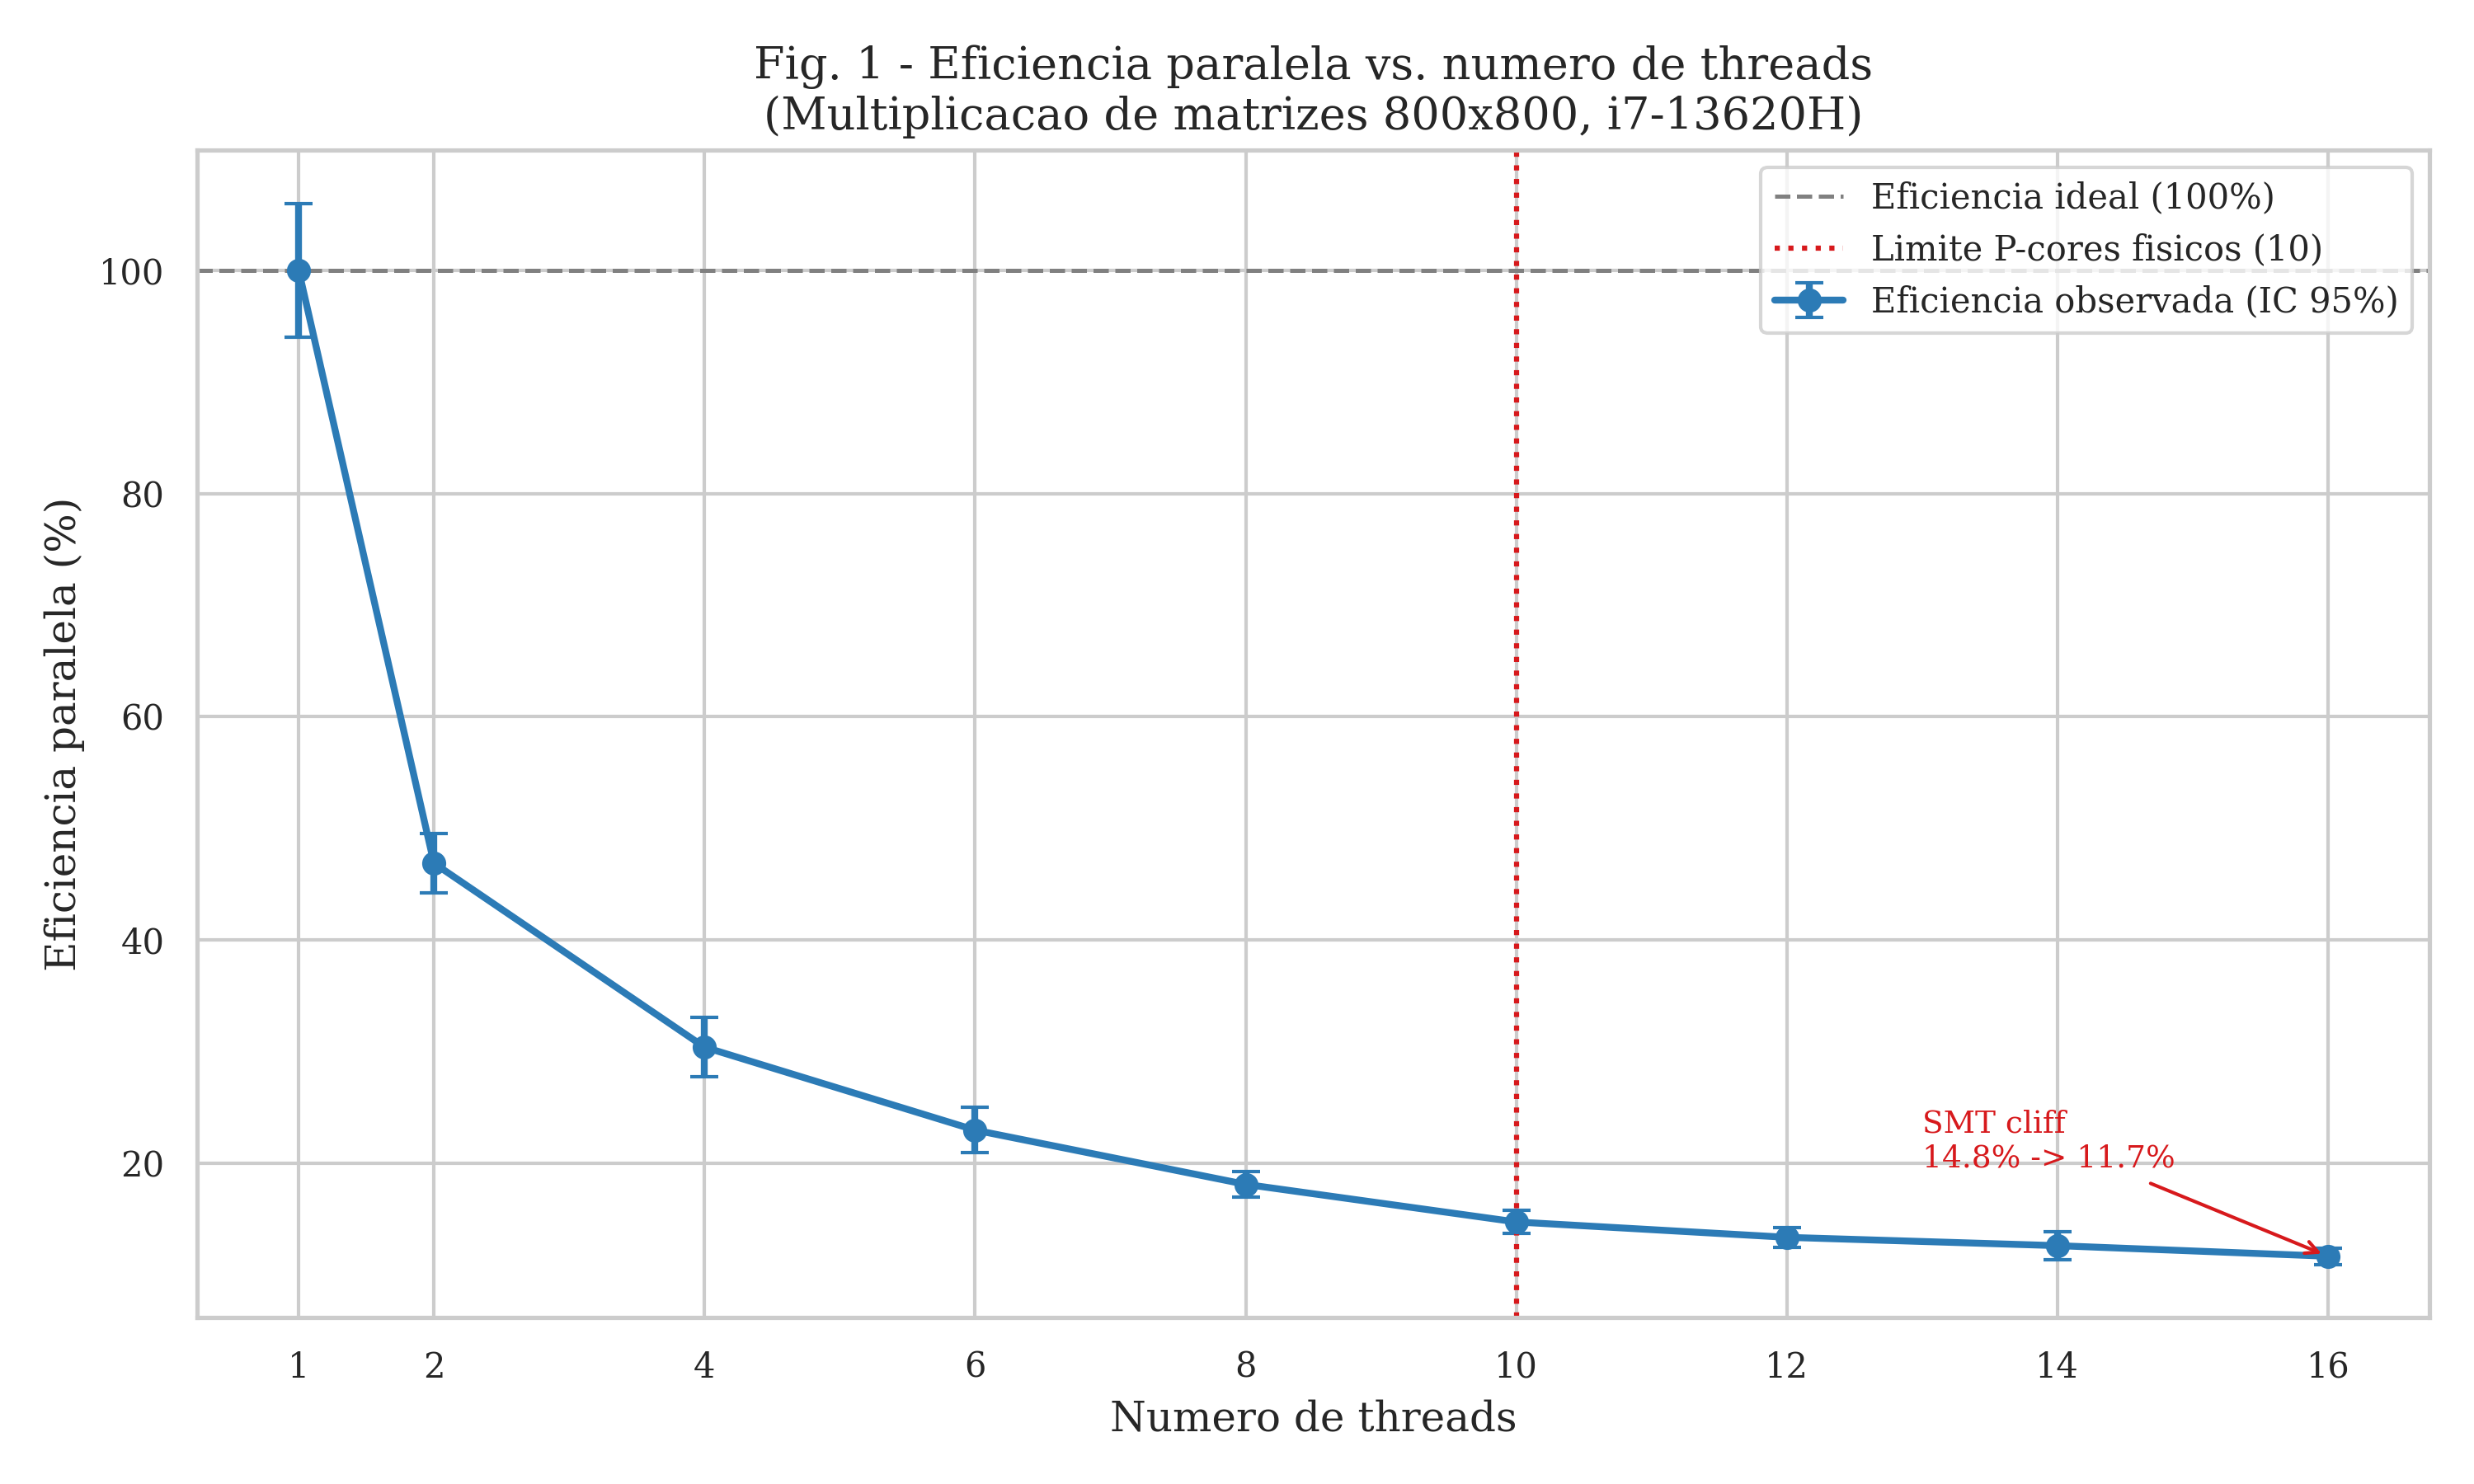
\includegraphics[width=0.85\textwidth]{figuras/fig1_eficiencia_threads.png}
\caption{Eficiência paralela vs.\ número de threads (multiplicação de matrizes
$800 \times 800$). A linha vertical marca o limite de 10 P-cores físicos.}
\label{fig:efic}
\end{figure}

\begin{figure}[ht]
\centering
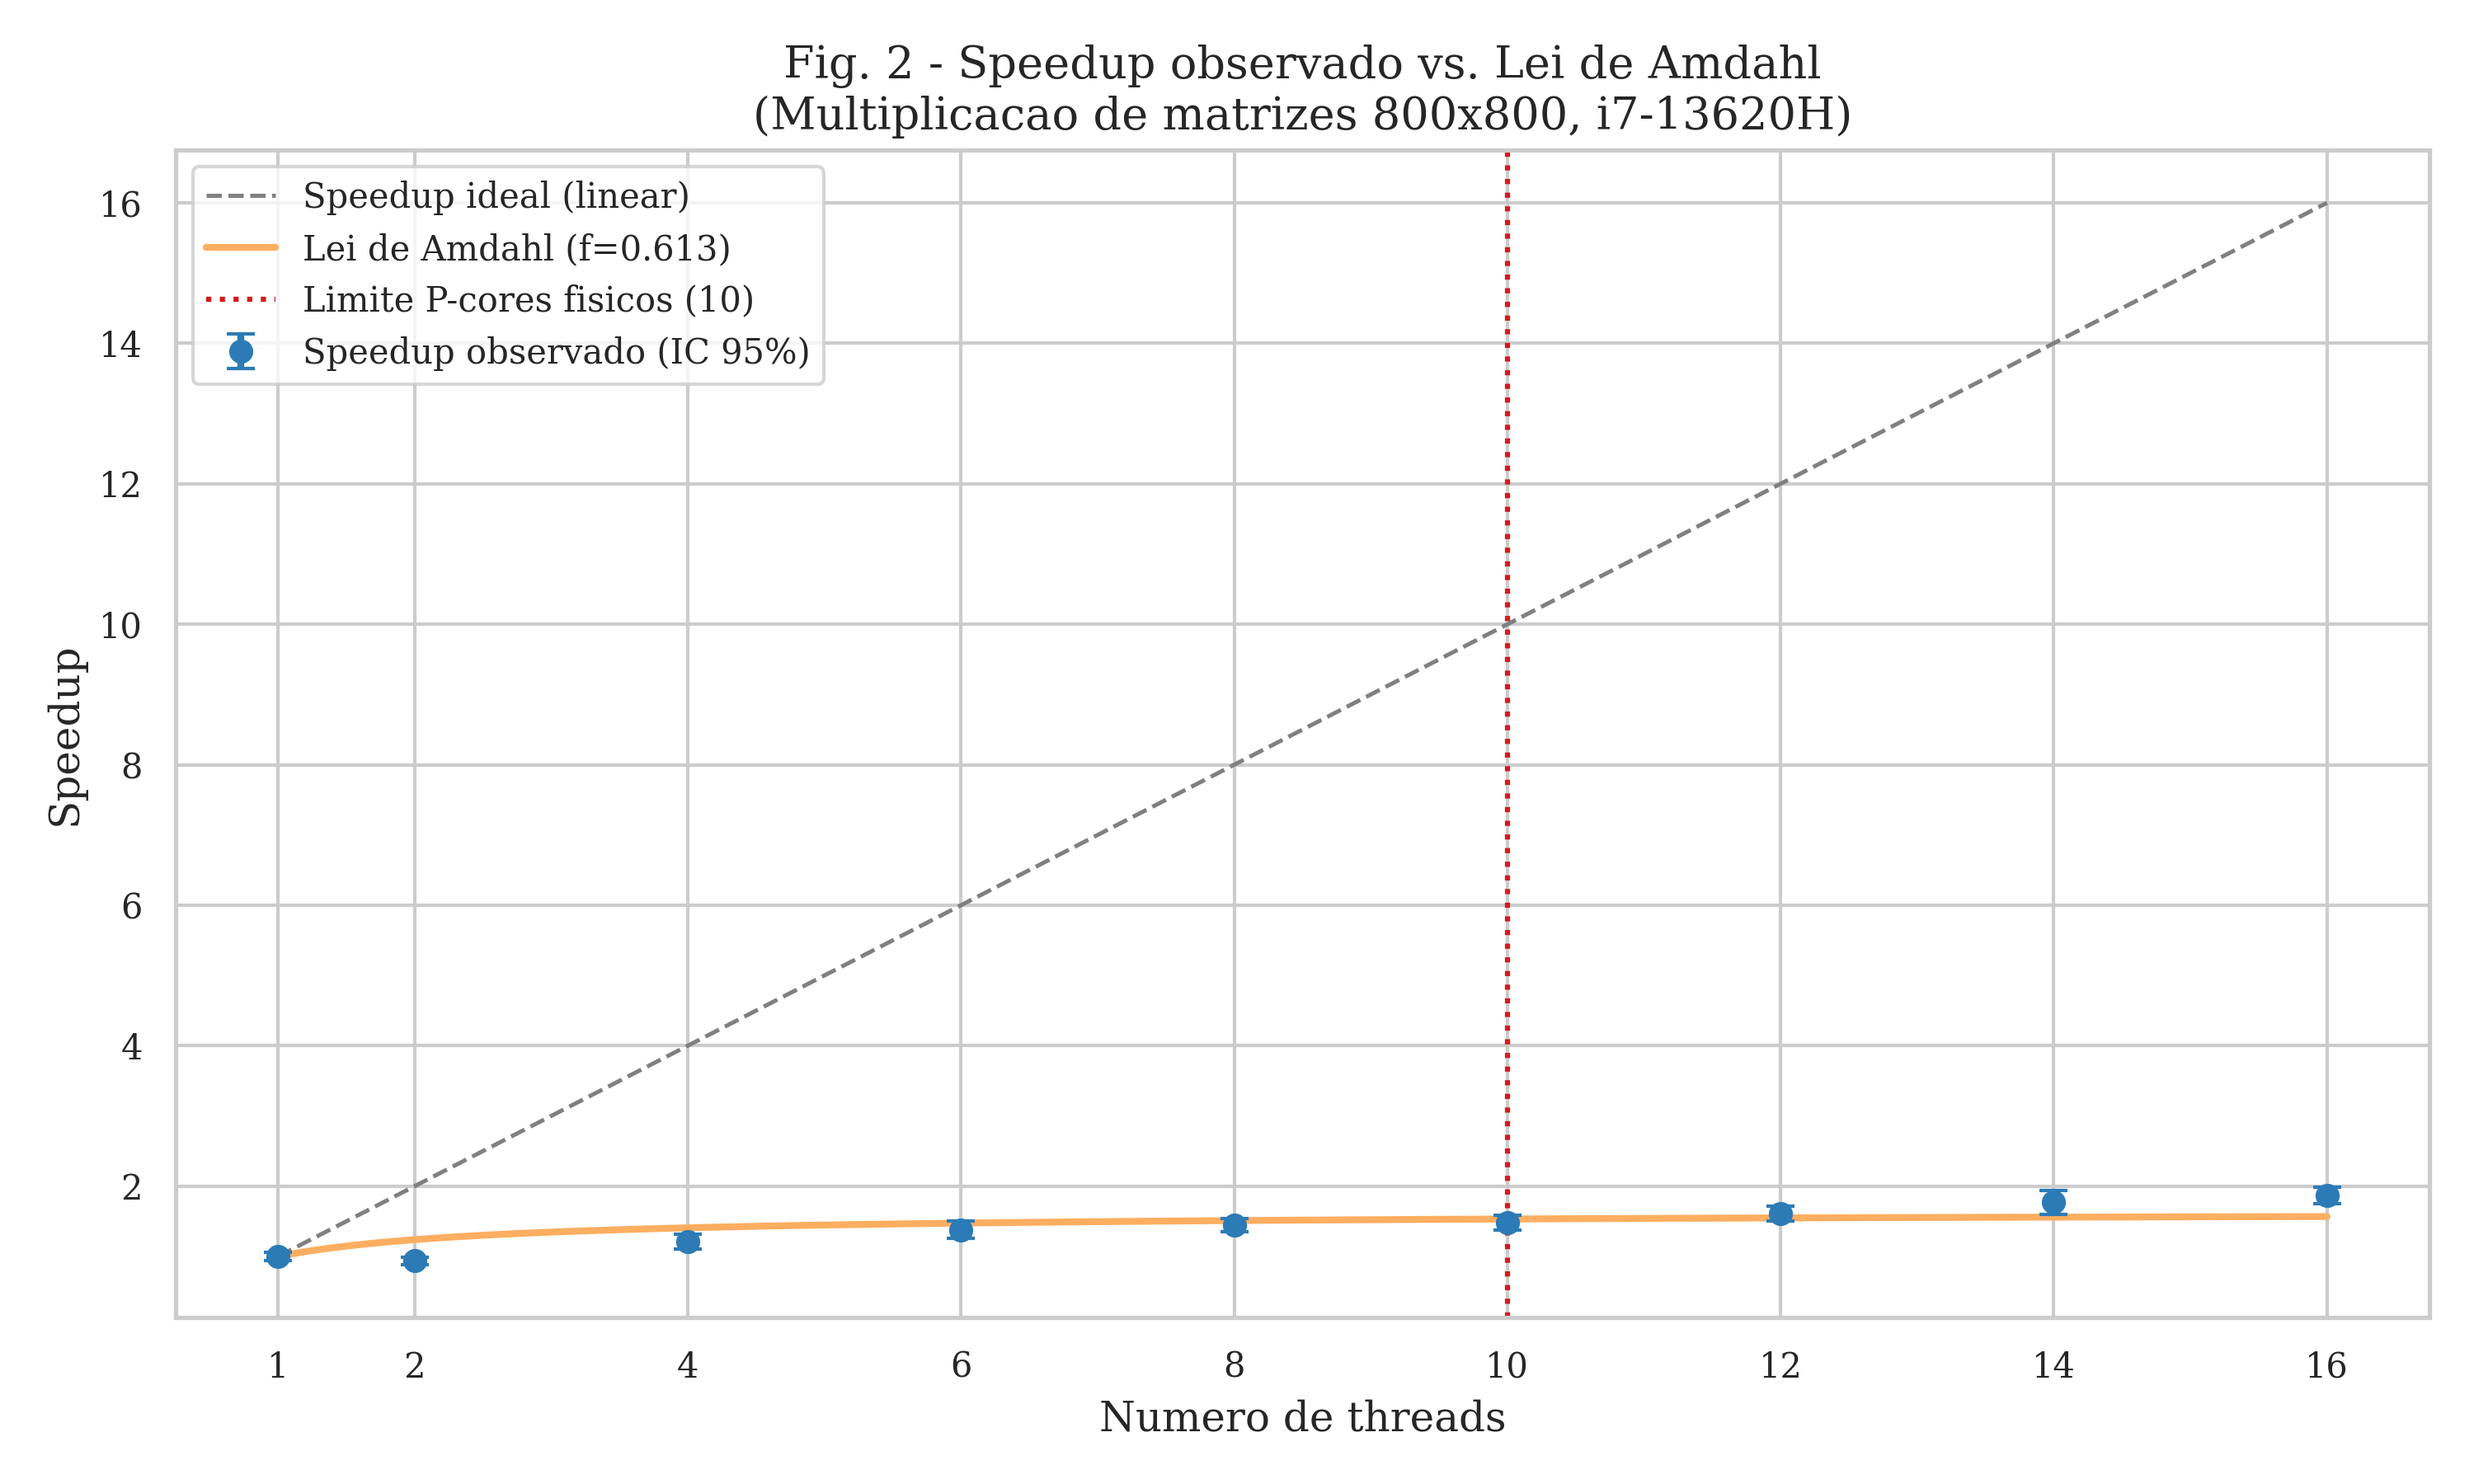
\includegraphics[width=0.85\textwidth]{figuras/fig2_speedup_amdahl.png}
\caption{Speedup observado vs.\ Lei de Amdahl com fração serial $f$ estimada por
mínimos quadrados.}
\label{fig:speedup}
\end{figure}

\subsection{Experimento B: sysbench CPU (strong scaling)}

\begin{table}[ht]
\centering
\caption{Experimento B --- sysbench CPU (strong scaling).}
\label{tab:expB}
\begin{tabular}{rrrrrr}
\hline
\textbf{Threads} & \textbf{Média (ev/s)} & \textbf{DP (ev/s)} & \textbf{IC 95\%} & \textbf{Speedup} & \textbf{Efic.\ (\%)} \\
\hline
1  & 1530,0  & 1,8  & [1529,3; 1530,6]   & 1,00 & 100,0 \\
2  & 3047,7  & 7,0  & [3045,0; 3050,3]   & 1,99 & 99,6 \\
4  & 5913,1  & 6,0  & [5910,8; 5915,3]   & 3,86 & 96,6 \\
6  & 8866,1  & 5,9  & [8863,9; 8868,4]   & 5,80 & 96,6 \\
8  & 11401,0 & 31,2 & [11389,3; 11412,6] & 7,45 & 93,1 \\
10 & 13866,8 & 27,1 & [13856,7; 13876,9] & 9,06 & 90,6 \\
12 & 13831,1 & 83,5 & [13800,0; 13862,3] & 9,04 & 75,3 \\
14 & 13824,4 & 85,8 & [13792,4; 13856,5] & 9,04 & 64,5 \\
16 & 13870,0 & 66,5 & [13845,2; 13894,8] & 9,07 & 56,7 \\
\hline
\end{tabular}
\end{table}

O throughput cresce quase linearmente até 10 threads (speedup 9,06$\times$,
eficiência 90,6\%), mas estagna a partir desse ponto: com 12, 14 e 16 threads o
valor permanece praticamente idêntico ao de 10 threads. A
Figura~\ref{fig:throughput} detalha a curva de throughput em relação ao ideal
linear.

\begin{figure}[ht]
\centering
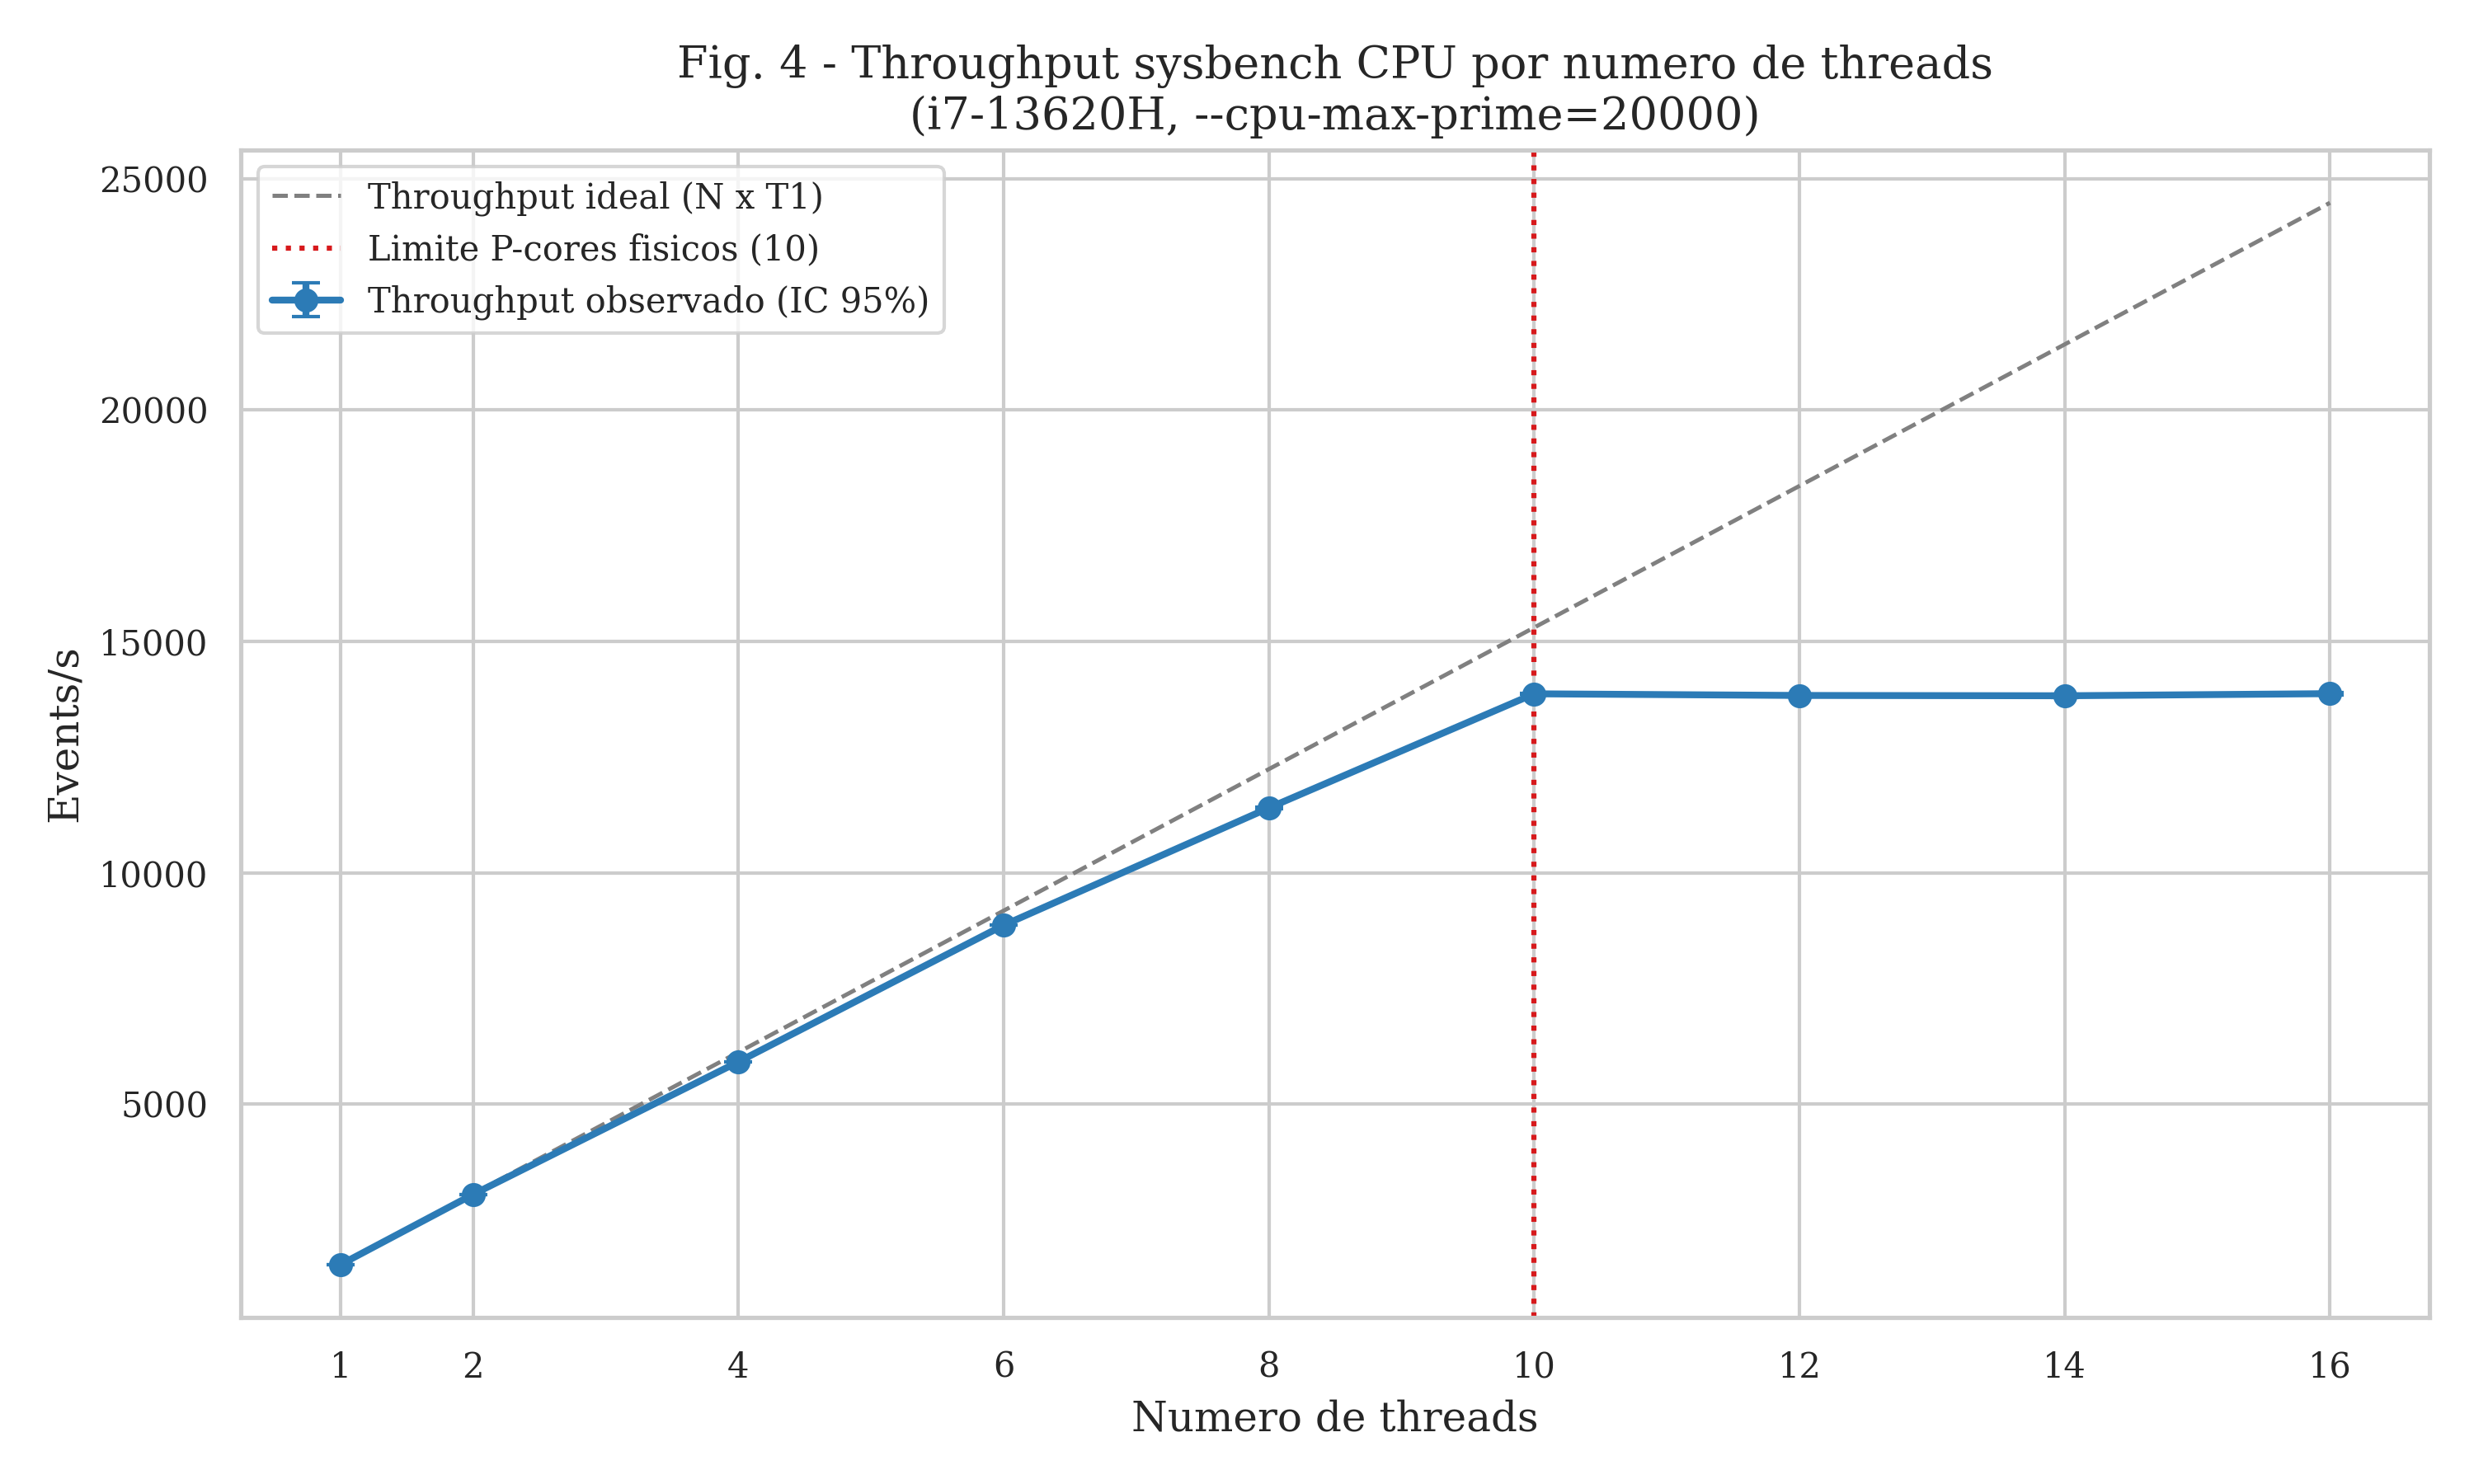
\includegraphics[width=0.85\textwidth]{figuras/fig4_sysbench_throughput.png}
\caption{Throughput do sysbench CPU vs.\ número de threads. O plateau a partir
de 10 threads evidencia a ausência de ganho do SMT em carga CPU-bound.}
\label{fig:throughput}
\end{figure}

\subsection{Testes de Hipótese}

\begin{table}[ht]
\centering
\caption{Testes de hipótese ($\alpha = 0{,}05$).}
\label{tab:hip}
\begin{tabular}{lllrrl}
\hline
\textbf{Métrica} & \textbf{Comparação} & \textbf{Teste} & \textbf{Estatística} & \textbf{p-valor} & \textbf{Rejeita H0?} \\
\hline
paralelismo & 1 vs.\ 10  & t pareado & $-89,77$   & $<0{,}001$ & sim \\
paralelismo & 1 vs.\ 10  & Wilcoxon  & $0,0$      & $<0{,}001$ & sim \\
paralelismo & 10 vs.\ 16 & t pareado & $-21,73$   & $<0{,}001$ & sim \\
paralelismo & 10 vs.\ 16 & Wilcoxon  & $0,0$      & $<0{,}001$ & sim \\
sysbench    & 1 vs.\ 10  & t pareado & $-2448,29$ & $<0{,}001$ & sim \\
sysbench    & 1 vs.\ 10  & Wilcoxon  & $0,0$      & $<0{,}001$ & sim \\
sysbench    & 10 vs.\ 16 & t pareado & $-0,25$    & $0,804$    & não \\
sysbench    & 10 vs.\ 16 & Wilcoxon  & $168,0$    & $0,191$    & não \\
\hline
\end{tabular}
\end{table}

O resultado mais relevante é o do sysbench, 10 vs.\ 16 threads: $p = 0{,}804$ (t
pareado) e $p = 0{,}191$ (Wilcoxon), de modo que não se rejeita H0 para o
throughput. Ou seja, adicionar threads via SMT (11--16) não melhora
significativamente o throughput. Por outro lado, a eficiência por thread cai de
90,6\% para 56,7\% --- degradação de 34,0 pontos percentuais ---, confirmando
H1 no quesito eficiência.

\section{Discussão}
\label{sec:discussao}

\subsection{Achado Principal: Plateau de Throughput por SMT}

O resultado mais claro é o plateau de throughput no sysbench a partir de 10
threads (limite dos P-cores físicos). De 10 para 16 threads o throughput varia
apenas 0,02\% --- variação não significativa ($p = 0{,}804$). Para cargas
puramente CPU-bound, o SMT no i7-13620H não contribui com capacidade
computacional adicional: os dois threads lógicos por P-core compartilham as
mesmas unidades de execução e competem por tempo de CPU sem que o pipeline
fique ocioso (ao contrário de cargas mistas). A degradação de eficiência é
consequência direta: o denominador cresce (mais threads), mas o numerador
(throughput) não. Em termos práticos, configurar um pool de threads igual ao
número de threads lógicas (16) em vez do número de P-cores (10) desperdiça 34,0
pontos percentuais de eficiência sem ganho de velocidade.

\subsection{Overhead de Processos Python (Weak Scaling)}

O Experimento A revelou que o overhead de criação de processos Python com o
método \texttt{spawn} ($\approx 0{,}1$--$0{,}2$ s por processo) supera o
benefício do paralelismo para tarefas de curta duração ($T_1 \approx 0{,}094$
s). Com 2 processos, o tempo total (0,201 s) é maior do que executar 2 tarefas
sequencialmente ($2 \times 0{,}094 = 0{,}188$ s), resultando em eficiência de
46,9\%. Em Python, \texttt{multiprocessing.Pool} com \texttt{spawn} é adequado
apenas para tarefas com duração significativamente maior que o overhead de
criação de processos.

\subsection{Contenção de Cache L3}

Cada processo no Experimento A aloca duas matrizes $800 \times 800$ de
\texttt{float64} ($\approx 5{,}1$ MB cada par). Com 4 processos,
$\approx 20{,}5$ MB de dados ativos --- próximo ao limite do L3 (24 MB). Com
10+ processos, os dados excedem o L3, forçando acessos à DRAM. Os dados de
largura de banda (Figura~\ref{fig:bw}, ferramenta mbw) ilustram a diferença de
banda entre os métodos de cópia e os tamanhos de bloco testados, indicando que
a hierarquia de cache é um fator relevante para a carga estudada. Ressalta-se,
contudo, que a contenção de L3 é aqui \emph{inferida} a partir da relação entre
o conjunto de trabalho e a capacidade do cache: não foram coletados contadores
de \emph{last-level cache miss} via \texttt{perf}, de modo que a quantificação
direta desse efeito permanece como trabalho futuro.

\begin{figure}[ht]
\centering
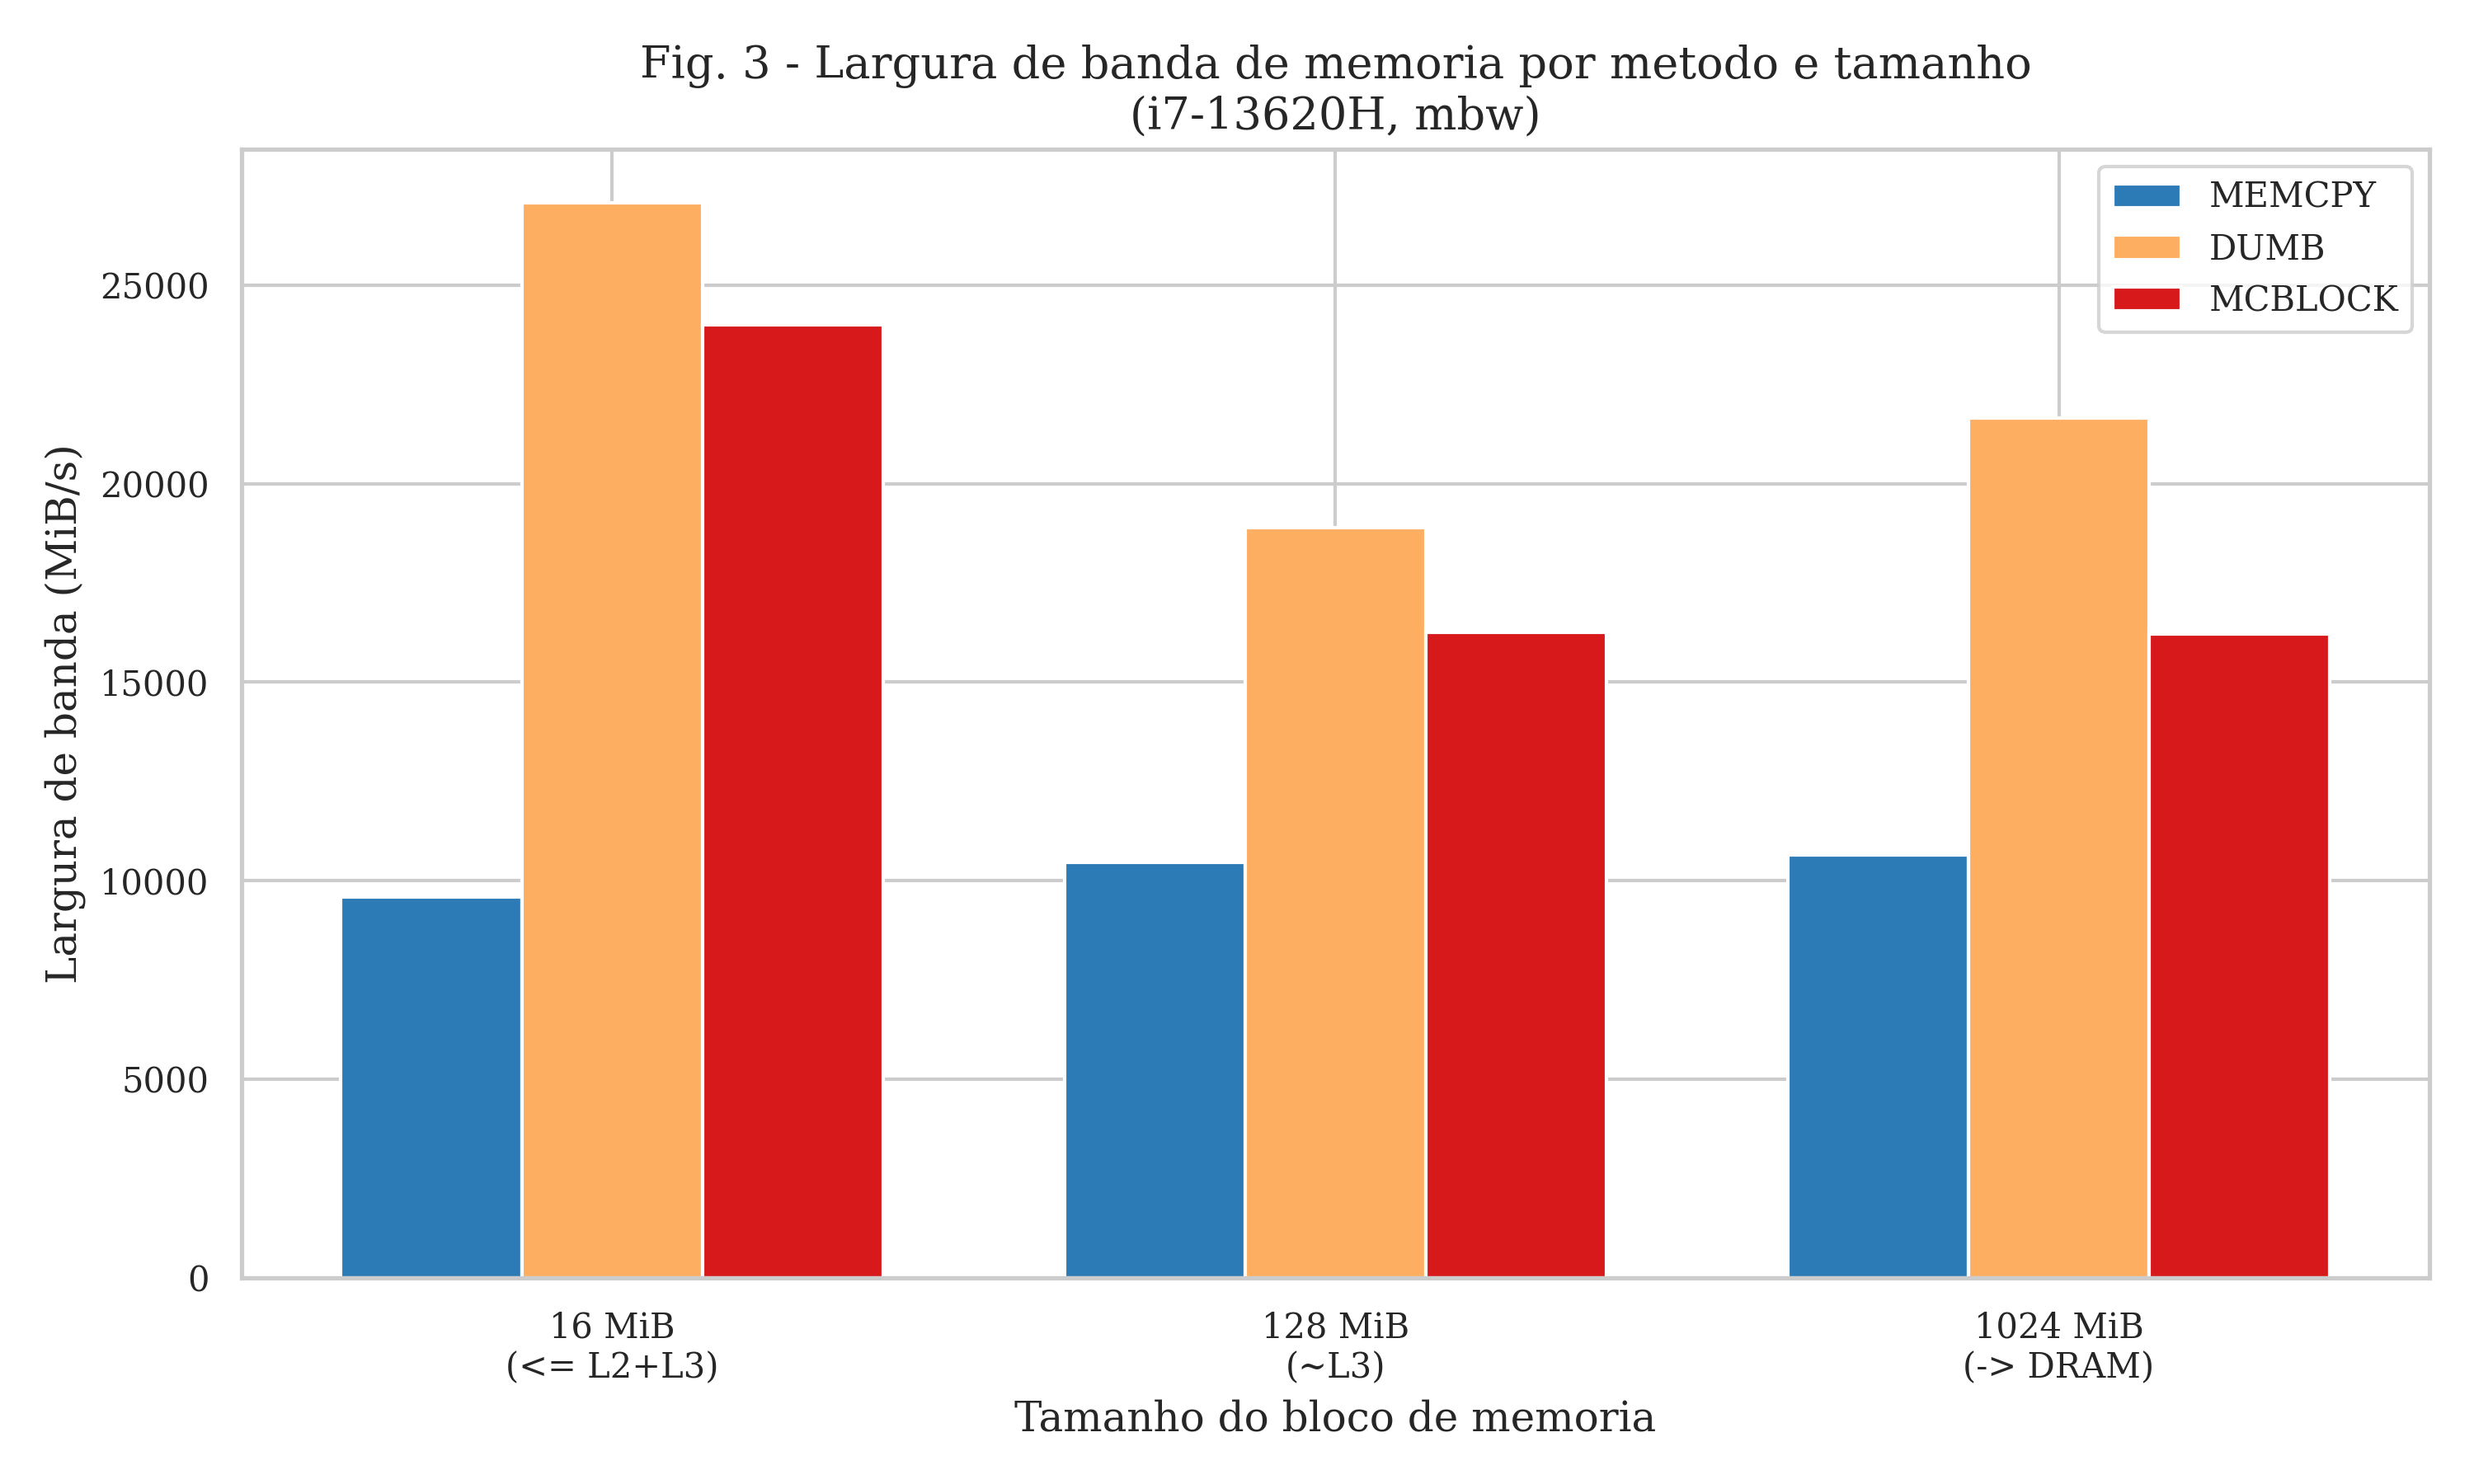
\includegraphics[width=0.85\textwidth]{figuras/fig3_bandwidth_cache.png}
\caption{Largura de banda de memória por método (mbw) e tamanho de bloco (16,
128 e 1024 MiB).}
\label{fig:bw}
\end{figure}

\subsection{Comparação com Dados Piloto}

Os dados piloto anteriores (governor \texttt{powersave}, sem repetições
formais) registravam anomalias em 16 threads. Os dados desta coleta confirmam o
padrão geral: a eficiência degrada progressivamente com o aumento de threads, e
esse é um resultado robusto, não um artefato do governor.

\subsection{Ameaças à Validade e Limitações}

\begin{itemize}
  \item \textbf{Única máquina:} sem comparação com AMD Zen 4 ou outra geração
  Intel; os resultados podem não generalizar para arquiteturas homogêneas.
  \item \textbf{Método spawn:} no Experimento A, o overhead de criação domina;
  resultados com \texttt{fork} seriam diferentes.
  \item \textbf{Contenção de L3 inferida:} o efeito de L3 é deduzido do
  conjunto de trabalho vs.\ capacidade do cache, não medido por contadores de
  hardware (\texttt{perf}).
  \item \textbf{Sem isolamento de CPU:} não foram usados \texttt{taskset}/
  \texttt{numactl}; o escalonador pode ter distribuído threads entre P-cores e
  E-cores de forma não determinística.
  \item \textbf{Turbo Boost:} pode elevar frequências de forma variável,
  introduzindo variabilidade mesmo com governor \texttt{performance}.
  \item \textbf{Dados de largura de banda:} a coleta com mbw é piloto (5
  execuções, poucos tamanhos), servindo de evidência complementar e não de
  medida principal.
\end{itemize}

\section{Conclusão}
\label{sec:conclusao}

Este estudo demonstrou empiricamente dois efeitos distintos no Intel Core
i7-13620H. Primeiro, o SMT não melhora o throughput em carga CPU-bound: o teste
sysbench confirma que adicionar threads via SMT (10 $\rightarrow$ 16) não
produz aumento significativo de throughput ($p = 0{,}804$), mas degrada a
eficiência por thread de 90,6\% para 56,7\%. Segundo, o overhead de criação de
processos Python domina em tarefas curtas: o método \texttt{spawn} do
\texttt{multiprocessing.Pool} introduz overhead que supera o benefício do
paralelismo para tarefas com $T_1 < 0{,}5$ s.

\textbf{Resposta à pergunta de pesquisa:} para cargas CPU-bound neste
processador, o SMT não melhora o throughput (H0 não rejeitada para throughput,
$p = 0{,}804$), mas degrada a eficiência por thread em 34,0 pontos percentuais
(H1 confirmada para eficiência). A recomendação prática é limitar pools de
processos/threads ao número de P-cores físicos (10 no i7-13620H), e não ao
total de threads lógicas.

Trabalhos futuros devem investigar: (i) comparação com o método \texttt{fork}
para isolar o custo de \texttt{spawn}; (ii) CPUs AMD Zen 4 (homogêneas) na mesma
carga; (iii) cargas mistas CPU+E/S em que o SMT pode apresentar ganhos; (iv)
medição direta da contenção de L3 com contadores de hardware (\texttt{perf});
e (v) isolamento via \texttt{taskset} para controlar a distribuição entre
P-cores e E-cores.

\section*{Disponibilidade de Artefatos}

Scripts, dados brutos (CSV), análises e figuras estão disponíveis publicamente
em: \url{https://github.com/RafaelCoutinhoLima/Artigo_De_Hardware}.

\section*{Uso de Ferramentas de IA}

Ferramentas de inteligência artificial foram utilizadas como apoio à redação,
formatação e revisão do texto. A coleta dos dados, a execução dos experimentos
e a análise dos resultados foram conduzidas e verificadas pelo autor.

\bibliographystyle{sbc}
\bibliography{referencias}

\end{document}
